\documentclass[]{article}
\usepackage{lmodern}
\usepackage{amssymb,amsmath}
\usepackage{ifxetex,ifluatex}
\usepackage{fixltx2e} % provides \textsubscript
\ifnum 0\ifxetex 1\fi\ifluatex 1\fi=0 % if pdftex
  \usepackage[T1]{fontenc}
  \usepackage[utf8]{inputenc}
\else % if luatex or xelatex
  \ifxetex
    \usepackage{mathspec}
  \else
    \usepackage{fontspec}
  \fi
  \defaultfontfeatures{Ligatures=TeX,Scale=MatchLowercase}
\fi
% use upquote if available, for straight quotes in verbatim environments
\IfFileExists{upquote.sty}{\usepackage{upquote}}{}
% use microtype if available
\IfFileExists{microtype.sty}{%
\usepackage{microtype}
\UseMicrotypeSet[protrusion]{basicmath} % disable protrusion for tt fonts
}{}
\usepackage[margin=1in]{geometry}
\usepackage{hyperref}
\hypersetup{unicode=true,
            pdftitle={Project2: Breast Cancer Prediction Model},
            pdfauthor={Group 7: Melanie Mayer, Yuqi Miao, Sibei Liu, Xue Jin},
            pdfborder={0 0 0},
            breaklinks=true}
\urlstyle{same}  % don't use monospace font for urls
\usepackage{graphicx,grffile}
\makeatletter
\def\maxwidth{\ifdim\Gin@nat@width>\linewidth\linewidth\else\Gin@nat@width\fi}
\def\maxheight{\ifdim\Gin@nat@height>\textheight\textheight\else\Gin@nat@height\fi}
\makeatother
% Scale images if necessary, so that they will not overflow the page
% margins by default, and it is still possible to overwrite the defaults
% using explicit options in \includegraphics[width, height, ...]{}
\setkeys{Gin}{width=\maxwidth,height=\maxheight,keepaspectratio}
\IfFileExists{parskip.sty}{%
\usepackage{parskip}
}{% else
\setlength{\parindent}{0pt}
\setlength{\parskip}{6pt plus 2pt minus 1pt}
}
\setlength{\emergencystretch}{3em}  % prevent overfull lines
\providecommand{\tightlist}{%
  \setlength{\itemsep}{0pt}\setlength{\parskip}{0pt}}
\setcounter{secnumdepth}{0}
% Redefines (sub)paragraphs to behave more like sections
\ifx\paragraph\undefined\else
\let\oldparagraph\paragraph
\renewcommand{\paragraph}[1]{\oldparagraph{#1}\mbox{}}
\fi
\ifx\subparagraph\undefined\else
\let\oldsubparagraph\subparagraph
\renewcommand{\subparagraph}[1]{\oldsubparagraph{#1}\mbox{}}
\fi

%%% Use protect on footnotes to avoid problems with footnotes in titles
\let\rmarkdownfootnote\footnote%
\def\footnote{\protect\rmarkdownfootnote}

%%% Change title format to be more compact
\usepackage{titling}

% Create subtitle command for use in maketitle
\providecommand{\subtitle}[1]{
  \posttitle{
    \begin{center}\large#1\end{center}
    }
}

\setlength{\droptitle}{-2em}

  \title{Project2: Breast Cancer Prediction Model}
    \pretitle{\vspace{\droptitle}\centering\huge}
  \posttitle{\par}
    \author{Group 7: Melanie Mayer, Yuqi Miao, Sibei Liu, Xue Jin}
    \preauthor{\centering\large\emph}
  \postauthor{\par}
      \predate{\centering\large\emph}
  \postdate{\par}
    \date{March 31, 2020}


\begin{document}
\maketitle

\hypertarget{introduction}{%
\subsection{Introduction}\label{introduction}}

Breast cancer is the most common invasive cancer and the second leading
cause of death from cancer in women worldwide, marked by the
uncontrolled growth of breast cells. Non-cancerous breast tumors do not
metastasize and are usually not life-threatening, while malignant tumors
are cancerous, aggressive and deadly. Therefore, it's important to have
breast lumps accurately diagnosed so that decision with regard to
medical treatment, rehabilitation and personal matters can be made
appropriately.

\hypertarget{objectives}{%
\subsection{Objectives}\label{objectives}}

The main objective of this project is to build an accurate predictive
model based on logistic regression that classifies between malignant and
benign images of breast tissue. Using the Breast Cancer Diagnosis
dataset, logistics model and logistic-LASSO model will be implemented to
predict the diagnosis. A Newton-Raphson algorithm and Pathwise
Coordinate optimization will be developed to estimate the logistic model
and the lasso model respectively. We aim to find the model with the best
performance in terms of predicting when breast tissue is malignant.

\hypertarget{breast-cancer-diagnosis-dataset}{%
\subsection{Breast Cancer Diagnosis
Dataset}\label{breast-cancer-diagnosis-dataset}}

The Breast Cancer Diagnosis dataset contains the diagnosis and a set of
10 features capturing the characteristics of the cell nuclei present in
the digitized image of breast mass. The ten features collected for each
cell nucleus are:

\begin{itemize}
\tightlist
\item
  radius (mean of distances from center to points on the perimeter)
\item
  texture (standard deviation of gray-scale values)
\item
  perimeter
\item
  area
\item
  smoothness (local variation in radius lengths)
\item
  compactness (perimeter\^{}2 / area - 1.0)
\item
  concavity (severity of concave portions of the contour)
\item
  concave points (number of concave portions of the contour)
\item
  symmetry
\item
  fractal dimension (``coastline approximation'' - 1)
\end{itemize}

The mean, standard deviation (SD) and largest values of these features
are computed for each image, resulting in 30 possible predictive
variables. We will analyze the predictive ability for diagnosis of
malignant or benign cases of these covariates. The mean of each feature
will be included in our models and presented in the result section. We
will also create models with all 30 predictors however, these results
will be reported in the supplement section.

\hypertarget{methods}{%
\subsection{Methods}\label{methods}}

\hypertarget{model-parameters}{%
\subsubsection{Model Parameters}\label{model-parameters}}

For logistic regression we assume the response variable \(Y_i\) for the
\(i_{th}\) observation follows a binary distribution:

\[Y_i\sim Bin(\pi_i)\] where \(\pi_i\) denotes the probablity that the
\(i_{th}\) observation's tissue is malignant. We can assume all
observations are independent from one another, hence the likelihood
function for the vector \(\boldsymbol\pi\) can be written as:

\[L(\boldsymbol\pi)=\prod_{i=1}^n f(y_i)=\prod_{i=1}^n\pi_i^{y_i}(1 - \pi_i)^{1-y_i}\]

For logistic regression, the logit link function is used:
\[\log(\frac{\pi_i}{1-\pi_i}) = \boldsymbol \beta ^T\boldsymbol x_i = \theta_i\]
where
\(\boldsymbol x_i^T = \begin{bmatrix} 1 & x_{1i} &x_{2i} & ... & x_{pi} \end{bmatrix}\)
and
\(\boldsymbol \beta^T = \begin{bmatrix} \beta_0 & \beta_1 & \beta_2 & ... & \beta_p \end{bmatrix}\).
One can solve for \(\pi_i = \frac{e^{\theta_i}}{1 + e^{\theta_i}}\). We
aim to find the best estimate of the vector of coefficients,
\(\boldsymbol \beta\). The log-likelihood function for this vector can
be written as:

\[l(\boldsymbol\theta)=logL(\boldsymbol\pi) =\sum_{i=1}^n(Y_ilog\frac{\pi_i}{1-\pi_i}+log(1-\pi_i)) = \sum_{i=1}^n(Y_i\theta_i - log(1 + e^{\mathbf \theta_i}))\\\]
The maximum likelihood is thus achieved when the gradient is equal to
zero and the Hessian is negative definite. The gradient can be found to
be:

\[\nabla l(\boldsymbol\theta|\boldsymbol X) = \sum_{i=1}^n (Y_i - \pi_i)\boldsymbol x_i = \boldsymbol X^T(\boldsymbol Y - \boldsymbol \pi) \]

The Hessian matrix is thus:

\[\nabla^2 l(\boldsymbol\theta|\boldsymbol X) = -\sum_{i=1}^n \pi_i(1 - \pi_i)\boldsymbol x_i\boldsymbol x_i^T = -\boldsymbol X^Tdiag(\pi_i(1 - \pi_i)) \boldsymbol X\]

\hypertarget{full-model}{%
\subsubsection{Full model}\label{full-model}}

In order to estimate \(\boldsymbol \beta\) we need to maximize the
loglikelihood function. There is no closed form, hence we turn to
numerical methods. The Newton-Raphson method is used to fit the full
logistic model. To find the maximum likelihood estimate of each element
of \(\boldsymbol \beta\), an iterative process is set as follows:

\[\theta_{i+1}  = \theta_{i} -\delta (\nabla^2l(\theta_{i}|\boldsymbol X)-\gamma I)^{-1}\nabla l(\theta_{i}|\boldsymbol X) \]
This is the Newton-Raphson method with two modifications. \(\delta\) is
included in the process to accomplish the step-halving modification, the
step coefficient ensures the likelihood is always increasing in order to
achieve quicker convergence. Once the likelihood approaches convergence
the steps become smaller until convergence is reached. \(\gamma\) is the
modification coefficient to ensure the aescent direction of the
iteration vector at \(\theta_{i}\).

\hypertarget{logit-lasso-pathwise-coordinate-wise-update-algorithm}{%
\subsubsection{Logit-lasso pathwise coordinate-wise update
algorithm}\label{logit-lasso-pathwise-coordinate-wise-update-algorithm}}

In the case of large dimensionality of predictors or multicollinearity
it can be beneficial to perform a regularization method which shrinks
coefficients and can perform variable selection. Here we implement the
Least Absolute Shrinkage and Selection Operator (LASSO) method for
logistic regression with a path-wise coordinate-wise optimization
algorithm to select variables from the full model, increase the
prediction efficiency and avoid overfitting. With the large model, we
have 30 predictors describing 10 features, hence we are likely to
experience multicollinearity and expect LASSO to outperform the
classical logistic regression.

In LASSO we add an L1 penalization term to the squared loss function,
such that we try to find the coefficients to minimize:

\[min _{(\boldsymbol \beta)}\{-l({\boldsymbol \beta})+\lambda\sum_{j=0}^{p}|\beta_j| \}\]
With the pathwise coordinate-wise update algorithm, we find the
likelihood to be:
\[l({\boldsymbol \beta}) = -\frac{1}{2n}\sum_{i=1}^{n}\omega_i(z_i-{\boldsymbol {X_i\beta}})^2\]
where,
\[\pi_i = \frac{exp({\boldsymbol {X_i\beta}})}{1+exp({\boldsymbol {X_i\beta}})}\]

\[\omega_i = \pi_i(1-\pi_i)\]

\[z_i = {\boldsymbol {X_i\beta}}+\frac{y_i-\pi_i}{\pi_i(1-\pi_i)}\]

One must pre-define the tuning parameter sequence
\(\{\lambda_1,...,\lambda_s\}\) and a starting vector
\({\boldsymbol{\beta_{start=}}}\{\beta_0^{(0)},...,\beta_p^{(0)}\}\). To
imptove efficienct, it is best to define
\(max{(\boldsymbol \lambda)} = max(\boldsymbol\beta)\) where
\(\boldsymbol\beta\) refers to the estimated coefficients from the
previous iteration. The optimal process for each \(\lambda_u\) is then
found by using the optimal \(\boldsymbol {\beta_{u-1}}\) from the
previous iteration as a warm start. Within every iteration find the
optimal \(\beta\) coordinate-wise, that is minimize over one parameter
at a time while keeping all others fixed.

For \(\beta_j\) in \(t_{th}\) iteration

\[\beta_j^{(t)} = \left\{\begin{array}{lc} \frac{\sum_{i=1}^{n} \omega_i(z_i-\sum_{j=1}^{p}{\boldsymbol {X_i}\beta_j})}{\sum_{i}^{n}\omega_i},&j=0\\\frac{s(\beta_j^{(t*)},\lambda_un)}{\sum_{i=1}^{n}\omega_ix_{ij}^2},&j = 1,2,...,p\end{array}\right.\]

\[\beta_j^{(t*)} = \sum_{i=1}^{n}\omega_ix_{ij}z_{ij}^*\]
\[z_{ij}^* = z_i-\underset {\beta_k\neq0}{\sum_{k = 0}^{j-1}}\beta_k^{(i)}x_{ik}-\underset {\beta_k\neq0}{\sum_{k=j+1}^{p}}\beta_k^{(i-1)}x_{ik}\]

\hypertarget{cross-validation}{%
\paragraph{Cross Validation}\label{cross-validation}}

In order to check the model performance, we use 5-fold cross validation.
Using training dataset to choose the best tuning parameter and fit
model, and using test dataset to evaluate the final prediction. The
statistics we use to compare the validation is SSE and pearson
chi-square statistics, which are defined as:

\[SSE = \sum_{i=1}^{n}(y_i-{\widehat \pi_i})^2\]
\[{\widehat \pi_i} = log\frac{exp({\boldsymbol X_i\beta})}{1+exp({\boldsymbol X_i\beta})}\]
\[G = \sum_{i=1}^{n}\frac{y_i-{\widehat \pi_i}}{{\widehat \pi_i}(1-{\widehat \pi_i})}\]

By taking average of above 2 statistics of 5 fold, we get the final
index to evaluate the model fitting.

\hypertarget{results}{%
\subsection{Results}\label{results}}

\hypertarget{newton-raphson}{%
\subsubsection{Newton-Raphson}\label{newton-raphson}}

After doing the Newton-Raphson modified with step and direction, the
estimation of 10 coefficients of means are in table 1 which are
consistant with the results from glm function. When mean, SD and largest
values of 30 features are included, the estimation of all 30 features
are in Supplementary table1.

\begin{center}
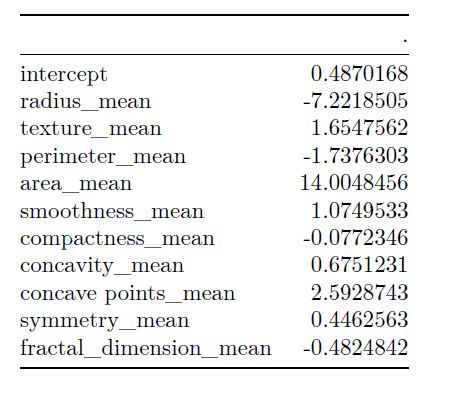
\includegraphics{./results/NR.JPG}
\end{center}

\begin{center}
Table 1. Estimated coefficients of 10 mean features under Newton-Raphson method
\end{center}

\hypertarget{coordinate-wise}{%
\subsubsection{Coordinate-Wise}\label{coordinate-wise}}

The range of \(\lambda\) we tried is (3,0) with length 100. The initial
guess of all \(\beta\) including the intercept is 0.02. The
g.statistics, SSE, AUC are introduced to select best \(\lambda\) in
Cross Validation. The optimal \(\lambda\) would be selected based on the
minimum SSE, maxmimum AUC and minimum g-statistics in test data. Below
is the results in 5-Fold Cross Validation:

\begin{center}
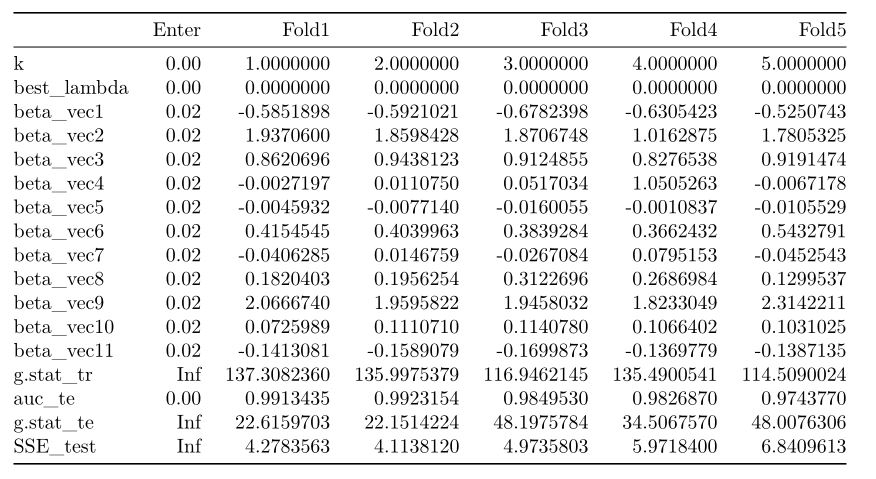
\includegraphics{./results/Results from Yuqi.JPG}
\end{center}

\begin{center}
Table 2. Cross validatin results in each fold
\end{center}

In all 5 folds, all three critria indicates the same optimal
\(\lambda\), whcih is 0. In the test data of each fold, the AUC ranges
from 0.99 to 0.97, g-statistics ranges from 22.6 to 48.0, while SSE
changes from 4.1 to 6.8.

\begin{center}
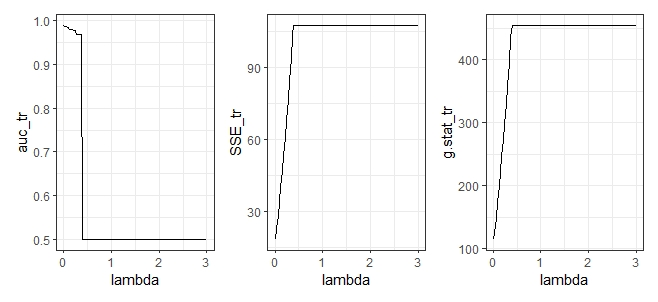
\includegraphics{./results/lambda_change.jpeg}
\end{center}

\begin{center}
Fig 1. Changes in three criteria vs $\lambda$
\end{center}

The Figure 1 shows the trend of AUC SSE and g-statistics in train data.
With the increse of \(\lambda\), both SSE and g-statistics have a
dramatic soar. While AUC has a great drop from 1 to 0.5. All of them
indicate that the bigger the \(\lambda\) is, the worse the model would
perform.

Since the optimal \(\lambda\)=0, none of the coefficients of
logistic-lasso is shrank into 0 as in Table 3.

\begin{center}
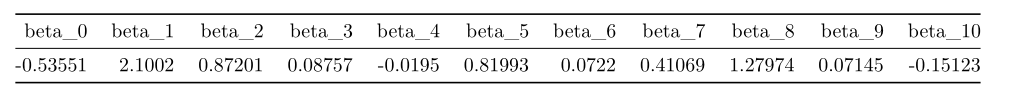
\includegraphics{./results/10 coed when lambd=0.png}
\end{center}

\begin{center}
Table 3. Coefficients in final model in Cross Validation
\end{center}

If total 30 features are considered, the corresponding Cross Validation
results in each fold is in Supplementary table2. The optimal \(\lambda\)
under that scenario is 0.03, which shrinks about 20 coefficients into 0
as presented in Supplementary table3.

\hypertarget{discussion}{%
\subsection{Discussion}\label{discussion}}

\hypertarget{supplementary}{%
\subsection{Supplementary}\label{supplementary}}

\begin{center}
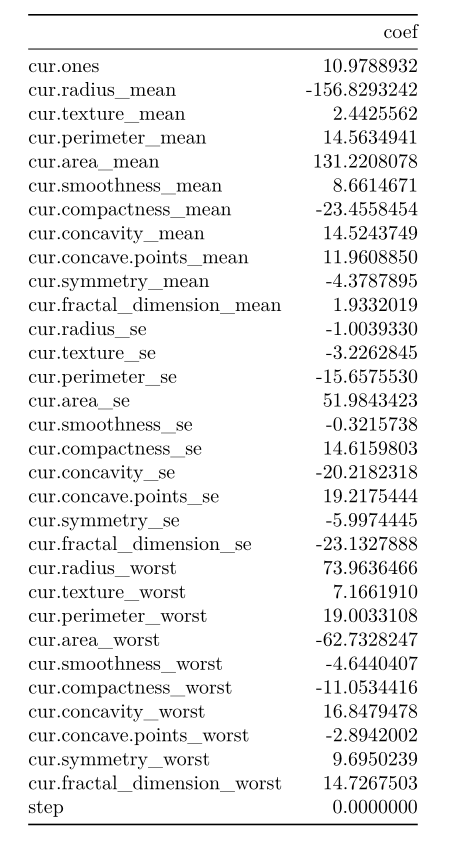
\includegraphics{./results/coef in NR of all 30 predictors.png}
\end{center}

\begin{center}
Supplementary Table1: Estimated coefficients of 30 features under Newton-Raphson method
\end{center}

\begin{center}
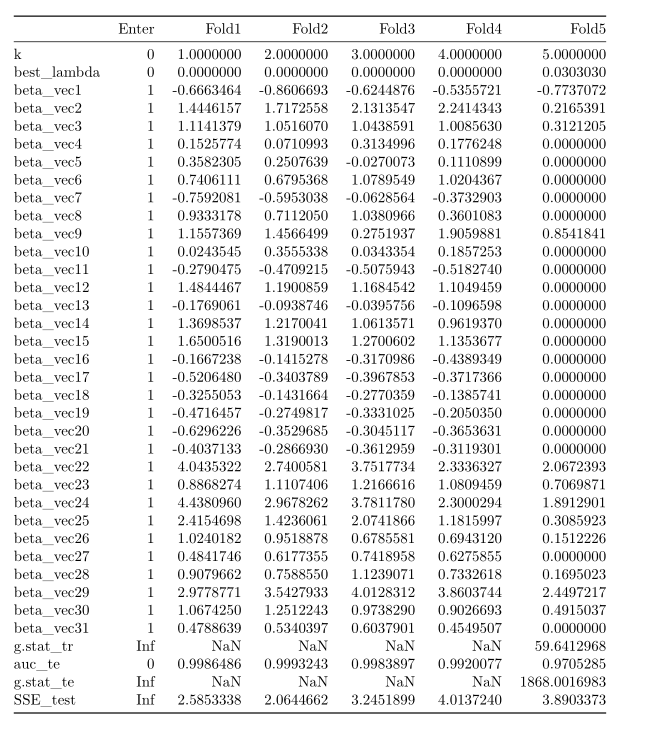
\includegraphics{./results/coef of all 30 predictors in logistic lasso.png}
\end{center}

\begin{center}
Supplementary Table2: Estimated coefficients of 30 features in each fold of Cross Validation
\end{center}

\begin{center}
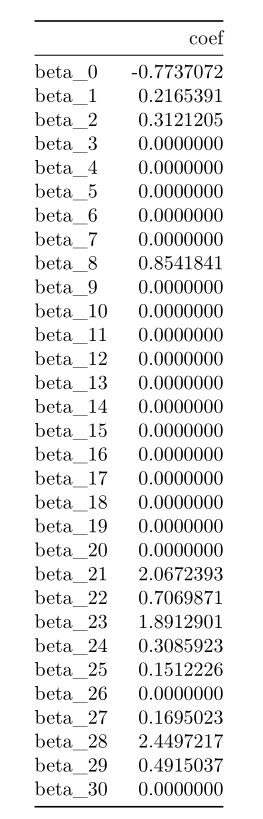
\includegraphics{./results/30 coefs when lambda=0.03.png}
\end{center}

\begin{center}
Supplementary Table3: Estimated coefficients of 30 features in final model in Cross Validation
\end{center}


\end{document}
